\documentclass[../mathNotesPreamble]{subfiles}
\begin{document}
%\relscale{1.4} %TODO
\section{13.4: Cross Products}
  \begin{defn*}[Cross Product]
    Given two nonzero vectors $\vecu$ and $\vecv$ in $\bbr^3$, the \textbf{cross product $\vecu\times\vecv$} is a vector with magnitude
      \[\abs{\vecu\times \vecv}=\abs{\vecu}\abs{\vecv}\sin\theta,\]
    where $0\leq \theta\leq \pi$ is the angle between $\vecu$ and $\vecv$. 

    The direction of $\vecu\times\vecv$ is given by the \textbf{right-hand rule}: 
    \begin{quote}
      When you put your the vectors tail to tail and let the fingers of your right hand curl from $\vecu$ to $\vecv$, the direction of $\vecu \times\vecv$ is the direction of your thumb, orthogonal to both $\vecu$ and $\vecv$ (Figure 13.56).
    \end{quote}
    
    When $\vecu\times \vecv=\bfO$, the direction of $\vecu\times\vecv$ is undefined.
  \end{defn*}
  \vspace*{\stretch{1}}
  \begin{center}
    \begin{minipage}{0.15\linewidth}
      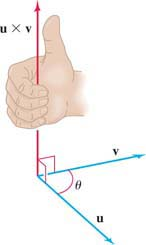
\includegraphics[width=\linewidth]{../images/briggs_13_04/fig13_56}
    \end{minipage}%
    \hspace*{0.25\linewidth}
    \begin{minipage}{0.3\linewidth}
      \begin{tikzpicture}[line width=1.5pt, scale=1.5]
        \coordinate (O) at (0,0);
        \coordinate (A) at (1.5,2);
        \coordinate (B) at (3,0);
        
        \draw[dashed, line width=1pt, black!50] (A) -- ($(A)+(B)$) -- (B);
        \draw[dashed, line width=1pt, black!50] (A) -- ($(O)!(A)!(B)$);
        \tkzFillAngle[draw= ClemsonOrange!90,size=0.45cm, opacity=0.8](B,O,A);
        \tkzLabelAngle[pos = 0.6,font=\normalsize](B,O,A){\color{black}$\theta$};
        \draw[ClemsonOrange, ->] (O) -- (A)
          node[above left,pos=0.5, black, font=\large] {$\vecv$};
        \draw[ClemsonPurple, ->] (O) -- (B) 
          node[above,pos=0.35, black, font=\large] {$\vecu$};
        \draw[black, <->, line width=0.9pt] ($(A)+(0.65,0)$)  -- node[pos=0.5, fill=white, inner sep=1pt, font=\large] {$\abs{\vecv}\sin\theta$} ($(O)!(A)!(B)+(0.65,0)$);
        \draw[black, <->, line width=0.9pt] ($(O)+(0,-0.25)$)  -- node[pos=0.5, fill=white, inner sep=1pt, font=\large] {$\vecu$} ($(B)+(0,-0.25)$);
      \end{tikzpicture}
    \end{minipage}
  \end{center}
  \vspace*{\stretch{1}}
  
  \begin{thmBox*}[Theorem 13.3: Geometry of the Cross Product]
    Let $\vecu$ and $\vecv$ be two nonzero vectors in $\bbr^3$.
    \begin{enumerate}
      \item 
        The vectors $\vecu$ and $\vecv$ are parallel ($\theta=0$ or $\theta=\pi$) if and only if $\vecu\times \vecv=\bfO$.
      \item 
        If $\vecu$ and $\vecv$ are two sides of a parallelogram, then the area of the parallelogram is
          \[\abs{\vecu\times \vecv}=\abs{\vecu}\abs{\vecv}\sin\theta\]
    \end{enumerate}
  \end{thmBox*}
  \pagebreak

  \begin{ex*}
    Consider the vectors $\vecu=\bracket{2,0,0}$ and $\vecv=\bracket{\sqrt3,3,0}$. The angle between these vectors is $\theta=\frac{\pi}{3}$. Find the area of the parallelogram formed by these vectors.
  \end{ex*}
  \vspace*{\stretch{1}}
  
  \begin{thmBox*}[Theorem 13.4: Properties of the Cross Product]
    Let $\vecu$, $\vecv$, and $\vecw$ be nonzero vectors in $\bbr^3$, and let $a$ and $b$ be scalars.
    \begin{center}
      \TabPositions{0.5\linewidth}
      \begin{enumerate}
        \item 
          $\vecu\times\vecv=-\parens{\vecv\times\vecu}$ 
          \tab \textcolor{blue}{Anticommutative property}
        \item 
          $\parens{a\vecu}\times\parens{b\vecv}=ab\parens{\vecu\times\vecv}$
          \tab \textcolor{blue}{Associative property}
        \item 
          $\vecu\times\parens{\vecv+\vecw}=\parens{\vecu\times\vecv}+\parens{\vecu\times\vecw}$
          \tab \textcolor{blue}{Distributive property}
        \item 
          $\parens{\vecu+\vecv}\times\vecw=\parens{\vecu\times\vecw}+\parens{\vecv\times\vecw}$
          \tab \textcolor{blue}{Distributive property}
      \end{enumerate}
    \end{center}
  \end{thmBox*}
  \pagebreak

  \begin{thmBox*}[Theorem 13.5: Cross Products of Coordinate Unit Vectors]
    \begin{align*}
      \bfi&\times\bfj= -\parens{\bfj\times\bfi}=\bfk& 
      \bfj&\times\bfk=-\parens{\bfk\times\bfj}=\bfi\\
      %
      \bfk&\times\bfi= -\parens{\bfi\times\bfk}=\bfj& 
      \bfi&\times\bfi=\bfj\times\bfj=\bfk\times\bfk=\bfO
    \end{align*}
  \end{thmBox*}
  \vspace*{2\baselineskip}
  
  \begin{minipage}{0.5\linewidth}
    \begin{center}
      \begin{tikzpicture}[scale=1.5]
        \begin{axis}[
          axis lines=center,
          axis line style={black,->},
          xmin=-1.25, xmax=2, xmajorticks=false,
          ymin=-1.25, ymax=2, ymajorticks=false,
          zmin=-1.25, zmax=2, zmajorticks=false,
          ticklabel style={font=\normalsize,inner sep=1pt,fill=white,opacity=1.0, text opacity=1},
          every axis plot/.append style={line width=0.95pt, color=blue, samples=100},
          view={130}{20},
          ]
          \draw[<->, black, line width=1pt] (0,0,-1) -- (0,0,1)
            node[right, font=\large, black, inner sep=2pt] {$\bfk$};
          \draw[<->, ClemsonPurple, line width=1pt] (-1,0,0) -- (1,0,0)
            node[pos=0.95, below, font=\large, black, inner sep=2pt] {$\bfi$};
          \draw[<->, ClemsonOrange, line width=1pt] (0,-1,0) -- (0,1,0)
            node[pos=0.95, below, font=\large, black, inner sep=2pt] {$\bfj$};
        \end{axis}
      \end{tikzpicture}
    \end{center}
  \end{minipage}%
  \begin{minipage}{0.5\linewidth}
    \begin{center}
      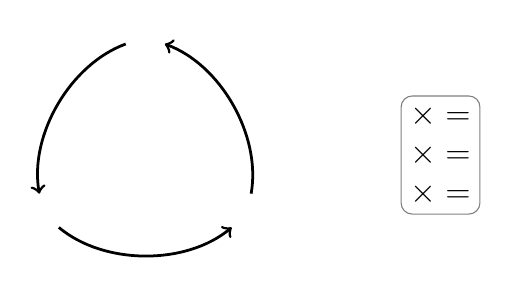
\begin{tikzpicture}[scale=1.5]
        \coordinate (i) at ({cos(210)},{sin(210)});
        \coordinate (j) at ({cos(-30)},{sin(-30)});
        \coordinate (k) at ({cos(90)},{sin(90)});
        
        \draw[->, shorten >=7.5pt, shorten <=7.5pt, line width=1pt] 
          (k) to[bend right=40] (i) node {$\bfi$};
        \draw[->, shorten >=7.5pt, shorten <=7.5pt, line width=1pt] 
          (i) to[bend right=40] (j) node {$\bfj$};
        \draw[->, shorten >=7.5pt, shorten <=7.5pt, line width=1pt] 
          (j) to[bend right=40] (k) node {$\bfk$};
        \node[align=left, rounded corners, draw=black!50, font=\large] at (2.5,0) {$\bfi\times\bfj=\bfk$\\$\bfj\times\bfk=\bfi$\\$\bfk\times\bfi=\bfj$};
      \end{tikzpicture}
    \end{center}
  \end{minipage}%
  \vspace*{\stretch{1}}

  \noindent
  Using the unit vectors, we can compute $\vecu\times\vecv$:
  \begin{align*}
    \vecu\times\vecv&= \parens{u_1\bfi+u_2\bfj+u_3\bfk}\times\parens{v_1\bfi+v_2\bfj+v_3\bfk}\\[0.75\baselineskip]
      &=u_1v_1\underbrace{\parens{\bfi\times\bfi}}_{\bfO}
       +u_1v_2\underbrace{\parens{\bfi\times\bfj}}_{\bfk}
       +u_1v_3\underbrace{\parens{\bfi\times\bfk}}_{-\bfj}\\
       %
      &+u_2v_1\underbrace{\parens{\bfj\times\bfi}}_{-\bfk}
       +u_2v_2\underbrace{\parens{\bfj\times\bfj}}_{\bfO}
       +u_2v_3\underbrace{\parens{\bfj\times\bfk}}_{\bfi}\\
       %
      &+u_3v_1\underbrace{\parens{\bfk\times\bfi}}_{\bfj}
       +u_3v_2\underbrace{\parens{\bfk\times\bfj}}_{-\bfi}
       +u_3v_3\underbrace{\parens{\bfk\times\bfk}}_{\bfO}\\
      &=\parens{u_2v_3-u_3v_2}\bfi
       -\parens{u_1v_3-u_3v_1}\bfj
       +\parens{u_1v_2-u_2v_1}\bfk
  \end{align*}
  \pagebreak

  \begin{thmBox*}[Theorem 13.6: Evaluating the Cross Product]
    Let $\vecu=u_1\bfi+u_2\bfj+u_3\bfk$ and $\vecv=v_1\bfi+v_2\bfj+v_3\bfk$. Then
    \[\vecu\times\vecv=
      \begin{vmatrix}
        \bfi& \bfj& \bfk\\
        u_1& u_2& u_3\\
        v_1& v_2& v_3
      \end{vmatrix}
      =\begin{vmatrix}
        u_2& u_3\\
        v_2& v_3
      \end{vmatrix}\bfi
      -\begin{vmatrix}
        u_1& u_3\\
        v_1& v_3
      \end{vmatrix}\bfj
      +\begin{vmatrix}
        u_1& u_2\\
        v_1& v_2
      \end{vmatrix}\bfk
    \]
    \textit{Note}:
      \[
      \begin{vmatrix}
        a&b\\c&d
      \end{vmatrix}
      =ad-bc
      \]
  \end{thmBox*}

  \[\vecu\times\vecv=\parens{u_2v_3-u_3v_2}\bfi
       -\parens{u_1v_3-u_3v_1}\bfj
       +\parens{u_1v_2-u_2v_1}\bfk\]
  
  \textbf{Alternative approach:}
    \begin{center}
      \begin{tikzpicture}
        [every node/.style={font=\LARGE, black}]
        \matrix (m){ 
          \node (i1) {$\bfi$};& \node (j1) {$\bfj$};& \node (k1) {$\bfk$};& 
          \node (i2) {$\bfi$};& \node (j2) {$\bfj$};\\
          \node (u11) {$u_1$};& \node (u21) {$u_2$};& \node (u31) {$u_3$};& 
          \node (u12) {$u_1$};& \node (u22) {$u_2$};\\
          \node (v11) {$v_1$};& \node (v21) {$v_2$};& \node (v31) {$v_3$};& 
          \node (v12) {$v_1$};& \node (v22) {$v_2$};\\
        };
        \draw[shorten <= -10pt, shorten >= -10pt] 
          ($(j1)!1.5!(i1)$) -- ($(v21)!1.5!(v11)$);
        \draw[shorten <= -10pt, shorten >= -10pt] 
          ($(k1)!0.5!(i2)$) -- ($(v31)!0.5!(v12)$);
        \draw[->, shorten <=-7.5pt, shorten >=-7.5pt] (u21) -- (v31);
        \draw[->, shorten <=-7.5pt, shorten >=-7.5pt] (u31) -- (v21);
        \draw[->, shorten <=-7.5pt, shorten >=-7.5pt] (u31) -- (v12);
        \draw[->, shorten <=-7.5pt, shorten >=-7.5pt] (u12) -- (v31);
        \draw[->, shorten <=-7.5pt, shorten >=-7.5pt] (u12) -- (v22);
        \draw[->, shorten <=-7.5pt, shorten >=-7.5pt] (u22) -- (v12);
      \end{tikzpicture}
    \end{center}

    \begin{ex*}
      Compute $\vecu\times\vecv$ for $\vecu=\bracket{3,5,4}$ and $\vecv=\bracket{1,-1,9}$.
    \end{ex*}
    \pagebreak

    \begin{ex*}
      Consider the vectors $\vecu=\bracket{\sqrt3,1,0}$ and $\vecv=\bracket{-\sqrt3,1,0}$. From the unit circle, we know the angle between these two vectors is $\theta=\frac{2\pi}{3}$. Use the definition of the cross product to show this.
    \end{ex*}
    \vspace*{\stretch{1}}

    \begin{ex*}
      Find the area of the triangle formed by $\vecu=\bracket{1,2,3}$ and $\vecv=\bracket{3,-1,1}$.
    \end{ex*}
    \vspace*{\stretch{1}}

    \pagebreak
  
    \begin{ex*}
      Given a force $\mathbf F$ applied to a point $P$ at the head of the vector $\vecr=\overrightharp{OP}$, the \textbf{torque} produced at point $O$ is given by $\mathbf \tau=\vecr\times\mathbf F$ with magnitude
        \[\abs{\mathbf \tau}=\abs{\vecr\times\mathbf F}=\abs{\vecr}\abs{\mathbf F}\sin\theta.\]
      Now suppose a force of $20 N$ is applied to a wrench attached to a bolt in a direction perpendicular to the bolt. Which produces more torque: applying the force at an angle of $60^\circ$ on a wrench that is $0.15 m$ long or applying the force at an angle of $135^\circ$ on a wrench that is $0.25 m$ long? 
      %TODO example about torque
    \end{ex*}
    \vspace*{\stretch{1}}
    \begin{center}
      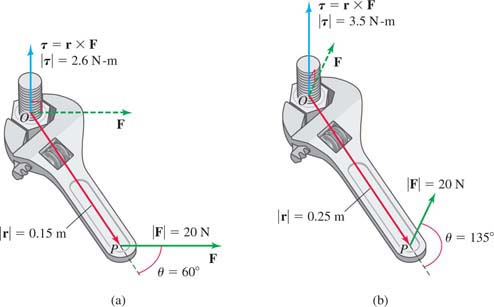
\includegraphics[width=0.75\linewidth]{../images/briggs_13_04/fig13_63}
    \end{center}

  \pagebreak
  
\end{document}